\documentclass[a4paper]{article}

\usepackage{fullpage} % Package to use full page
\usepackage{parskip} % Package to tweak paragraph skipping
\usepackage{tikz} % Package for drawing
\usepackage{amsmath}
\usepackage{amsthm}
\usepackage{amsfonts}
\usepackage{amssymb}
\usepackage{hyperref}
\usepackage{enumitem}

\newcommand{\norm}[1]{\left\lVert#1\right\rVert}
\newcommand{\abs}[1]{\left\lvert#1\right\rvert}

\newtheorem{lemma}{Lemma}

\everymath{\displaystyle}

\title{Data Mining: Homework 3}
\author{Anxhelo Xhebraj \\
        \href{mailto:xhebraj.1643777@studenti.uniroma1.it}{\texttt{xhebraj.1643777@studenti.uniroma1.it}}
        }
\date{ \{26 Nov .. 9 Dec\} 2018}

\begin{document}

\maketitle

\subsection*{Problem 2}

We will now study some questions of $k$-means on 1 dimension.

\begin{enumerate}
  \item Recall that in the $k$-means problem we want to minimize the total
    squared $\ell_2$ distance between each point and the center to which it is
    assigned to:
    \begin{align*}
      \sum_{i = 1}^{k} \sum_{x \in C_i} \norm{\mathbf{x} - \boldsymbol{\mu}_i}^2
    \end{align*}
    where $C_i$ is the set of points that belong to the $i$th cluster,
    $\boldsymbol{\mu}_i$ the mean of the points in the $i$th cluster, and
    \begin{align*}
      \norm{\mathbf{x}}^2 = \sum_{j = 1}^d x_j^2
    \end{align*}
    if $\mathbf{x} = (x_1, x_2, ..., x_d)$.

    In class, we said that in general the $k$-means problem is NP-hard. However,
    for $d$ = 1 the problem is polynomial. Design an algorithm that solves the
    $k$-means problem in time polynomial in the number of points $n$ and the
    number of clusters $k$, for $d$ = 1.

    (\textbf{Hint}: Can you solve the problem for $k$ clusters if you assume
    that you can solve it for fewer than $k$ clusters?)

    \textbf{Solution}: Let $X \subset \mathbb{R}, |X| = n$ be the set of points we want
    to cluster, denote by $\mathbf{x} = (x_1, x_2, ..., x_n)$ the sequence of
    elements in $X$ sorted by value and let $\mathbf{x}[i:j] = (x_i, x_{i + 1},
    ..., x_{j-1}) $.
    The problem of $k$-means for $d = 1$ can be rewritten as finding $k-1$ indices
    $i_1, i_2, ..., i_{k-1}$ that minimize
    \begin{align*}
      \phi_k(\mathbf{x}) &= \sum_{j = 0}^{k - 1} \phi(\mathbf{x}[i_j:i_{j +
      1}]), \qquad \text{with } i_0 = 1, \text{ } i_k = n
    \end{align*}

    where $\phi(\mathbf{y}), \mathbf{y} = (y_1, y_2, ..., y_m)$ is the
    contribute to the $k$-means cost of a sequence of points, i.e.
    
    \begin{align*}
      \phi(\mathbf{y}) &= \sum_{i = 1}^m \abs{y_i - \mu(\mathbf{y})}^2 \\
      \mu(\mathbf{y}) &= \frac{\sum_{i = 1}^m y_i}{m}.
    \end{align*}

    Note that this is equivalent to finding $k$ partitions that minimize the
    cost however we reduce the set of possible partitions to
    
    \begin{align*}
      \mathcal{P}(X) = \{P = (P_1, P_2, ..., P_k) | x_i
    \in P_o \land x_j \in P_o \land x_i < x_l < x_j \implies x_l \in P_o\}
    \end{align*}

    i.e. intervals of the $\mathbb{R}$ space.


    \begin{lemma}
      Let $P = (P_1, P_2, ..., P_k)$ be the optimal solution to the $k$-means
      problem for set $X = \{x_1, x_2, ..., x_n\}$ and let $x_i \in P_o$ and $x_j
      \in P_o$ with $x_i \neq x_j$. For any $x \in X$ such that $x_i < x <
      x_j$ then $x \in P_o$.
    \end{lemma}
    \begin{proof}
      Assume by contradiction $x \in P_p \neq P_o$. Given that $P$ is optimal
      then
      \begin{align*}
        \abs{x - \mu(P_p)}^2 < \abs{x - \mu(P_o)}^2
      \end{align*}
      Without loss of generality assume $x \geq \mu(P_o)$ then we have the
      following cases:
      \begin{enumerate}
        \item $\mu(P_o) < \mu(P_p) < x$: this would cotradict the hypothesis
          since by
        attaching $x_j$ to $P_p$ would lower the cost which by hyp was optimal.

        \item $ x < \mu(P_p) < x + \abs{x - \mu(P_o)} $ again assigning $x_j$ to
          $P_p$ would lower the cost contradicting the optimality hypothesis.
      \end{enumerate}
      The same holds for $x \le \mu(P_o)$ with $x_i$.
    \end{proof}

    The Lemma above shows that restricting the partitions to intervals leads to
    an optimal solution therefore the formulation above is correct.
    Now we can solve the problem by performing an exhaustive search over the
    possible values of $i_j$s.
    
    Assume we know the optimal cost
    $\phi_{h - 1}^*(\mathbf{x}[1:m])$, $\forall m$: $h - 1 < m \le n$ for some
    $h - 1 < k$. Then

    \begin{align*}
      \phi_{h}^*(\mathbf{x}[1:m]) = \min_{l = h}^m
      \phi_{h-1}^*(\mathbf{x}[1:l]) + \phi(\mathbf{x}[l:m]).
    \end{align*}
    
    i.e. if we know the optimal clustering of size $h-1$ for all
    prefixes of the points, we can derive the optimal clustering of size
    $h$.
    
    This is possible since minimizing $\phi_h(\mathbf{y})$ is equivalent to
    minimizing each $\phi(\mathbf{y}[i_{j}, i_{j + 1}])$ and once we know
    $\phi_{h-1}^*(\mathbf{y}[1:m]) = \min_m \phi_{h-1}(\mathbf{y}[1:m])$ for each $m$, what is left to choose is
    to which of the $m$ corresponds $i_{h-1}$ (the starting index of the
    last cluster) which minimizes the cost.

    We can compute a matrix $M$ where $M_{h,m} = \phi_h^*(\mathbf{x}[1:m])$
    computed as shown by the formula above except for the first row which is
    simply $\phi_1^*(\mathbf{x}[1:m]) = \phi(\mathbf{x}[1:m])$
    and another matrix $S$ keeping for
    each $M_{h,m}$ the index of the column in the previous row which minimized
    the cost in order to reconstruct the solution.

    \begin{align*}
      M &= 
      \begin{bmatrix}
        \phi_1^*(\mathbf{x}[1:1]) & \phi_1^*(\mathbf{x}[1:2]) &
        \phi_1^*(\mathbf{x}[1:3]) &\dots  & \phi_1^*(\mathbf{x}[1:n]) &
        \phi_1^*(\mathbf{x}[1:n + 1]) \\
        \bot & \phi_2^*(\mathbf{x}[1:2]) & \phi_2^*(\mathbf{x}[1:3]) & \dots &
        \phi_2^*(\mathbf{x}[1:n]) & \phi_2^*(\mathbf{x}[1:n + 1]) \\
        \bot & \bot & \phi_3^*(\mathbf{x}[1:3]) & \dots  &
        \phi_3^*(\mathbf{x}[1:n]) & \phi_3^*(\mathbf{x}[1:n + 1])\\
        \vdots & \vdots & \vdots & \ddots & \vdots & \vdots \\
        \bot & \bot & \bot & \dots  & \phi_k^*(\mathbf{x}[1:n]) &
        \phi_k^*(\mathbf{x}[1:n + 1])
      \end{bmatrix} \\
      S_{h,m} &= \arg \min_{l = h}^m
      \phi_{h-1}^*(\mathbf{x}[1:l]) + \phi(\mathbf{x}[l:m])
    \end{align*}
    
    Thus in order to solve the problem we need to compute the $S$ matrix and
    then find the indices by calling with parameters $k, n$ the following
    function: \\ Indices($k', n')\triangleq $\textbf{ if} $k > 1$:
    $\{S_{k',n'}\} \cup$
    Indices($k'-1, S_{k',n'} - 1$) \textbf{else}: $\emptyset $.

    \textbf{Cost analysis}: In order to compute the optimal indices as shown
    above the full $S$ matrix is needed therefore the cost in terms of space is
    in $O(kn)$. The computation time of the algorithm is in $O(kn^3)$ since
    the time for computing each cell of the matrix is in $O(n^2)$. The latter
    cost can be reduced to be in $O(n)$ obtaining a computation time in
    $O(kn^2)$ observing that $\phi(\mathbf{x}[l:m])$ can be computed once in a
    given row using any online algorithm for the Total Sum of Squares (or
    Corrected Sum of Squares). We overlooked the cost of sorting the points
    since it does not affect the computation time in Big-O notation.

  \item We are given a set $P$ of $n$ points in $\mathbb{R}$. For simplicity,
    assume that $\mu(P) = 0$, that is, $\sum_{x \in P} x = 0$. Let $\norm{P}^2 =
    \sum_{x \in P} x^2$ be the optimal 1-means cost. Show that by adding
    carefully $O(1/\epsilon)$ centers, we can make the $k$-means cost at most
    $\epsilon \cdot \sum_{x \in P} x^2$.

    \textbf{Hint:} First show that by adding 2 centers at locations $-\ell$ and
    $\ell$, for an appropriate value of $\ell$, the cost decreases by a factor of
    3/4.

    \textbf{Solution}:
    Assume we add $1/2\epsilon$ pairs of \textit{symmetric} centers $\ell_1,
    \ell_2, ..., \ell_{1/2\epsilon}$ and $-\ell_1,
    -\ell_2, ..., -\ell_{1/2\epsilon}$ with $\ell_{i - 1} \le \ell_i$ and
    $\ell_i \ge 0, \forall i$  and denote
    by $P_i^+$ the set of points
    assigned to center $\ell_i$ and $P_i^-$ the ones assigned to $- \ell_i$.
    Also let $P_0$ be the set of points assigned to center $0$.
    Then we can write the cost as

    \begin{align*}
      &\phi =\sum_{x \in P_0} x^2 + \sum_{i = 1}^{1/2\epsilon}\sum_{x \in P_i^+}
      (x - \ell_i)^2 + \sum_{i = 1}^{1/2\epsilon}\sum_{x \in P_i^-} (x + \ell_i)^2 \\
      &=\sum_{x \in P_0} x^2 + \sum_{i = 1}^{1/2\epsilon}\sum_{x \in P_i^+} (x^2
      - 2x\ell_i + \ell_i^2)
      + \sum_{i = 1}^{1/2\epsilon}\sum_{x \in P_i^-} (x^2
      + 2x\ell_i + \ell_i^2)\\
      &=\sum_{x \in P} x^2 + \sum_{i = 1}^{1/2\epsilon}\sum_{x \in P_i^+} (
      - 2x\ell_i + \ell_i^2) + \sum_{i = 1}^{1/2\epsilon}\sum_{x \in P_i^-} (
      2x\ell_i + \ell_i^2)\\
      &=\norm{P}^2 + \sum_{i = 1}^{1/2\epsilon}\sum_{x \in P_i^+} (
      - 2x\ell_i + \ell_i^2) + \sum_{i = 1}^{1/2\epsilon}\sum_{x \in P_i^-} (
      2x\ell_i + \ell_i^2).
    \end{align*}
      We can observe that $\forall x \in P_i \land 1 \le i < 1/2\epsilon $
      holds $|x| \ge \frac{\ell_{i+1} + \ell_i }{2}$ and for $ i = 1/2\epsilon$,
      $|x|
      \ge \frac{l_i}{2}$ i.e. the points belonging to a center $i$ should be
      closer to center $i$ than $i + 1$ (preceding center). Given that in the
      sums above $\forall x \in P_i^+ \rightarrow -2x\ell_i \le 0$ and $\forall x
      \in P_i^- \rightarrow 2x\ell_i \le 0$ we can write

      \begin{align*}
        \phi &= \norm{P}^2 + \sum_{i = 1}^{1/2\epsilon}\sum_{x \in P_i^+} (
        - 2x\ell_i + \ell_i^2) + \sum_{i = 1}^{1/2\epsilon}\sum_{x \in P_i^-} (
        2x\ell_i + \ell_i^2) \\
        &\le \norm{P}^2 + \sum_{i = 1}^{1/2\epsilon - 1}\sum_{x \in P_i^+} (
        - 2 \left( \frac{\ell_{i+1} + \ell_i }{2} \right) \ell_i + \ell_i^2) +
        \sum_{i = 1}^{1/2\epsilon - 1 }\sum_{x \in P_i^-} (
        2 \left( - \frac{\ell_{i+1} + \ell_i }{2} \right) \ell_i + \ell_i^2) \\
        &= \norm{P}^2 - 2\sum_{i = 1}^{1/2\epsilon - 1}\sum_{x \in P_i^+} (\ell_i
        \ell_{i + 1}) \\
        &\le \norm{P}^2 - 2\sum_{i = 1}^{1/2\epsilon - 1} (\ell_i \ell_{i + 1}) \\
        &=\norm{P}^2 - \frac{\epsilon - 1}{2\epsilon - 1}\norm{P}^2 \sum_{i = 1}^{1/2\epsilon - 1} \frac{1}{i (i
        + 1)} \qquad \qquad \qquad \text{if } \ell_i = \frac{1}{i \sqrt2}
        (\norm{P}^2)^{\frac{1}{2}}\frac{\epsilon - 1}{2\epsilon - 1}\\
        &= \epsilon \norm{P}^2
      \end{align*}
\end{enumerate}

    \iffalse
    \begin{figure}[!htbp]
    \begin{center}
    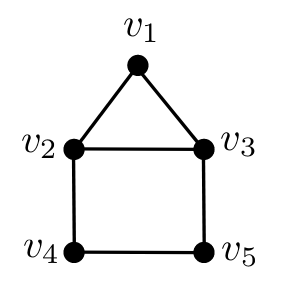
\includegraphics[width=70pt]{house.png}
    \end{center}
    \caption{\textit{The house subgraph}}\label{house}
    \end{figure}
    \fi

\end{document}
